% CC BY-NC-SA 3.0 (http://creativecommons.org/licenses/by-nc-sa/3.0/)

\documentclass{beamer}

\mode<presentation>{
\usetheme{Madrid}
}

\usepackage{graphicx}
\usepackage{booktabs}
\usepackage{adjustbox}
\usepackage{xcolor}
\usepackage{tikz}
\usepackage{animate}
\hypersetup{
  colorlinks=true,
  linkcolor=blue,
  urlcolor=blue,
  citecolor=blue
}

\newcommand{\positive}[1]{\textcolor{green!55!black}{#1}}
\newcommand{\negative}[1]{\textcolor{red!70!black}{#1}}
\definecolor{exampleText}{RGB}{0, 0, 180}
\definecolor{softTeal}{RGB}{22, 139, 130}

\title{TikZ Diagram Agent Skill}
\subtitle{Static Figures, Visual QA, and Animations}
\author{Workshop demo}
\institute{Agent-assisted research and teaching figures}
\date{\today}

\begin{document}

\begin{frame}
  \titlepage
\end{frame}

\section{What the Skill Tests}

\begin{frame}{Workflow the Skill Enforces}
  \begin{itemize}[<+->]
    \item Start from the communication job, not the decoration.
    \item Pick a figure grammar: axis/curve, DAG, tree, matrix, loop, corridor, or delayed path.
    \item Compile to PDF, render to PNG, and run static and rendered visual QA.
    \item Inspect the result: overlap, clipping, title-band collisions, crowding, and unclear teaching message.
    \item For animations, render a GIF or contact sheet so the frame sequence can be reviewed.
  \end{itemize}
\end{frame}

\begin{frame}{Prompt Shape}
  \small
  \begin{block}{User gives a sketch, paper figure, or teaching request}
    ``Create a TikZ version of this figure and animate the professor's likely build-up.''
  \end{block}
  \begin{block}{Agent response}
    Identify the figure grammar, decide what is worth animating, render, inspect, patch, and save checked artifacts.
  \end{block}
  \begin{block}{Output}
    \texttt{.tex}, \texttt{.pdf}, \texttt{.png}, visual-QA JSON, GIF/contact sheet, and a QA note.
  \end{block}
\end{frame}

\section{Sketch to Teaching Figure}

\begin{frame}{Input: Whiteboard-Style Macro Sketch}
  \small
  \begin{columns}[T,totalwidth=\textwidth]
    \begin{column}{0.45\textwidth}
      \textbf{Input request}
      \begin{itemize}
        \item Trace the photo as well.
        \item Preserve the classroom sketch grammar.
        \item Animate the AD shifts as multiplier rounds.
      \end{itemize}
    \end{column}
    \begin{column}{0.52\textwidth}
      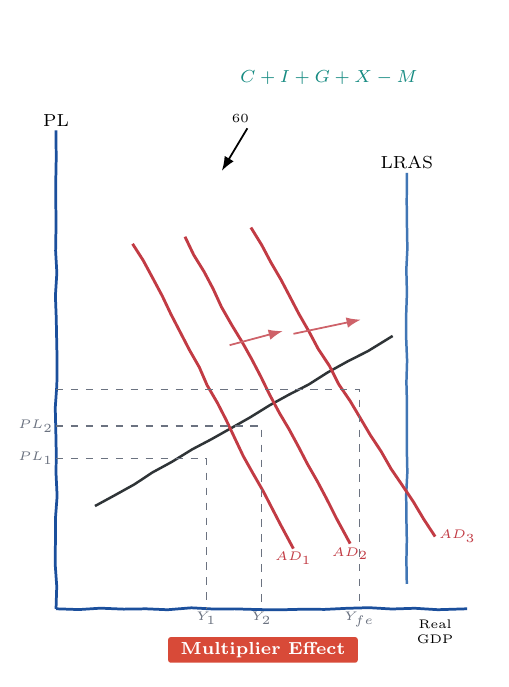
\includegraphics[width=\linewidth,height=0.72\textheight,keepaspectratio]{assets/multiplier_photo_trace.png}
    \end{column}
  \end{columns}
\end{frame}

\begin{frame}{Output: Multiplier Effect Animation}
  \centering
  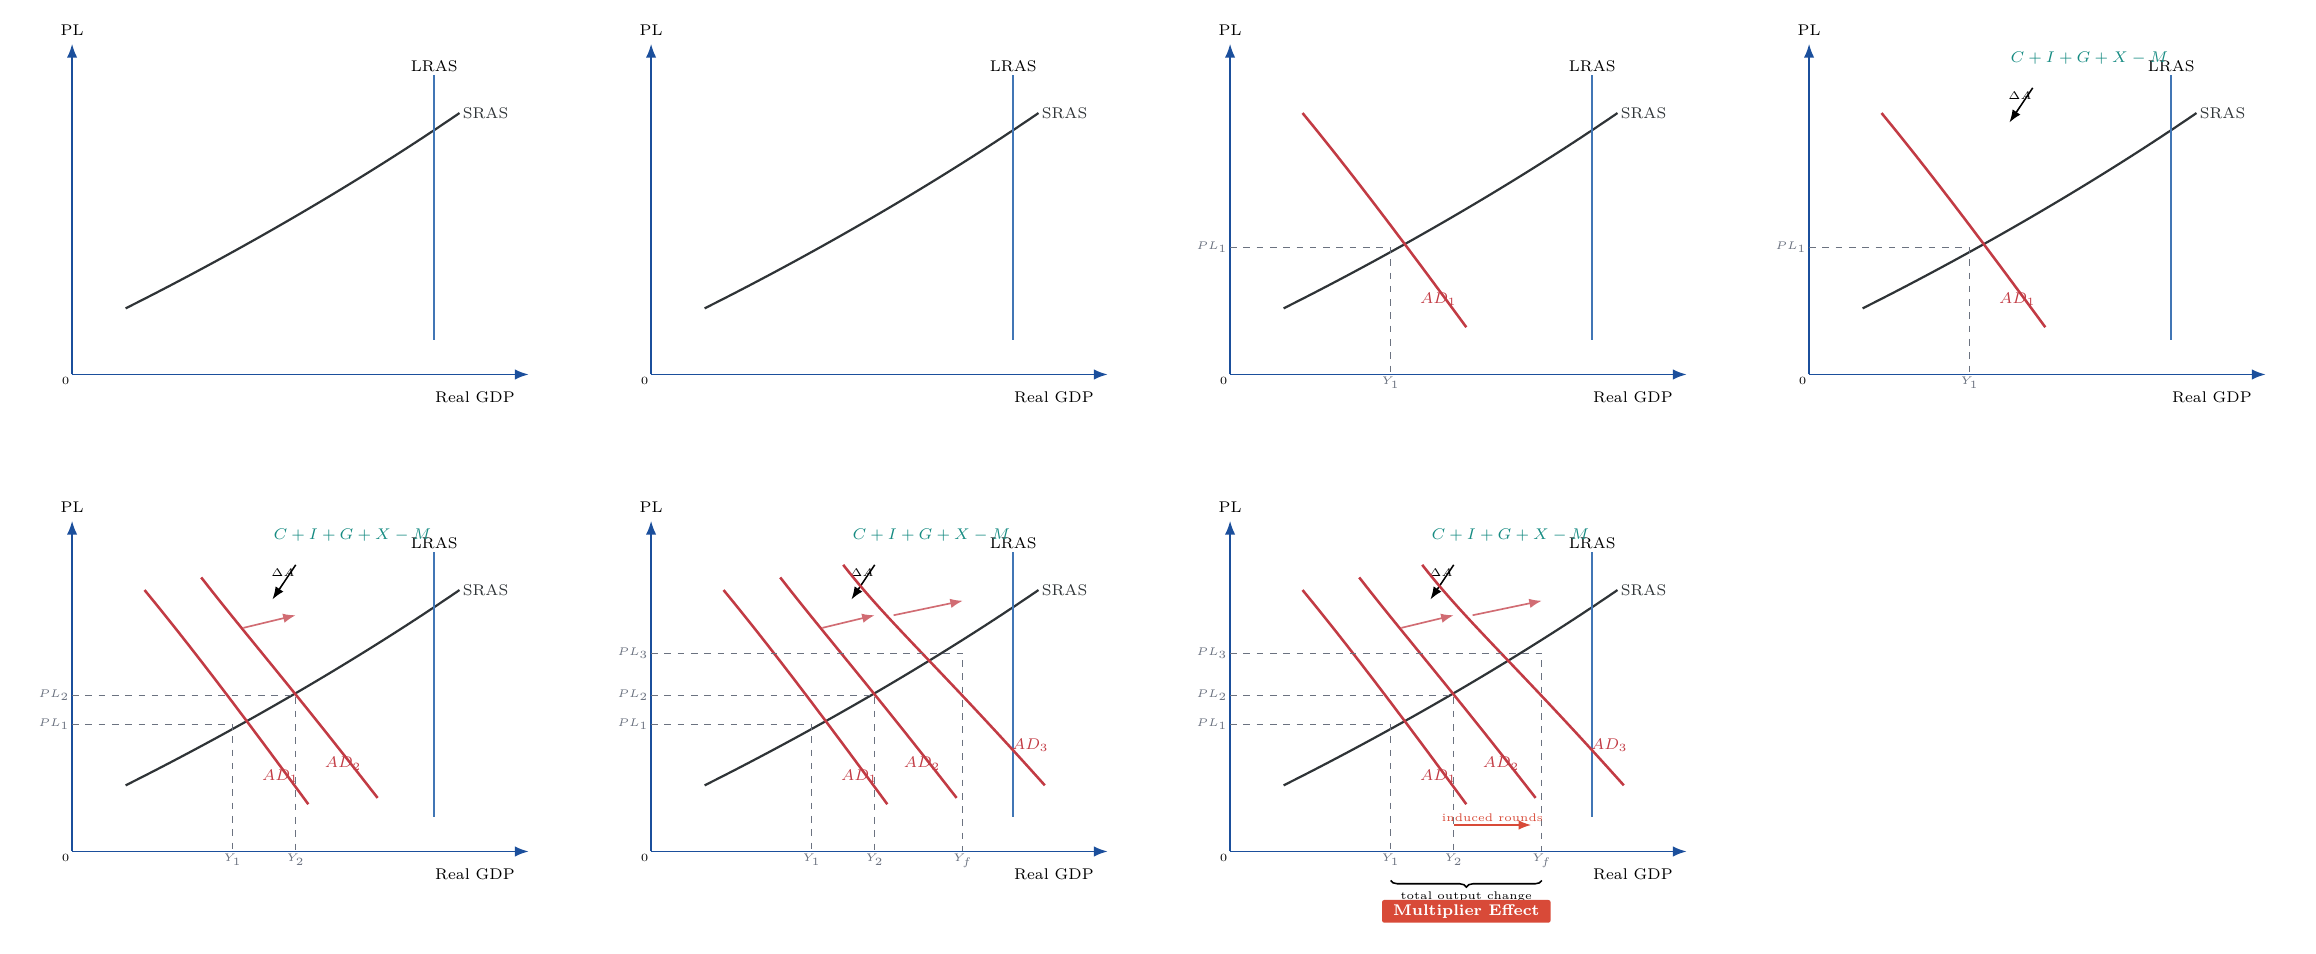
\includegraphics[width=\linewidth,height=0.68\textheight,keepaspectratio]{assets/multiplier_contact.png}

  \vspace{0.2cm}
  \small
  GIF preview: \href{run:assets/multiplier_animation.gif}{open local animation preview}
\end{frame}

\begin{frame}{PDF-Native Animation: Multiplier Effect}
  \centering
  \animategraphics[
    controls,
    loop,
    autoplay,
    width=\linewidth,
    height=0.70\textheight,
    keepaspectratio
  ]{6}{assets/multiplier_frames/frame-}{01}{44}

  \vspace{0.15cm}
  \small
  This uses \texttt{animate} plus PNG frames, so the animation is embedded in the PDF.
\end{frame}

\begin{frame}{Lesson: Trace and Clean Version Can Coexist}
  \begin{itemize}[<+->]
    \item A traced version preserves the professor's spatial memory.
    \item A clean animation makes the mechanism readable for students.
    \item The skill should reconstruct the teaching mechanism, not blindly trace every wobble.
    \item Visual QA caught edge-label problems before finalizing.
  \end{itemize}
\end{frame}

\section{Delayed Adjustment}

\begin{frame}{Input: J-Curve Teaching Prompt}
  \small
  \begin{block}{Prompt}
    Turn a rough phone-photo sketch of a current-account J-curve into a clean animated teaching figure.
  \end{block}
  \begin{itemize}
    \item Keep the portrait, quick-explainer feel.
    \item Show depreciation first, low short-run price elasticity, then long-run recovery.
    \item Do not put caption prose inside the image.
  \end{itemize}
\end{frame}

\begin{frame}{Output: J-Curve Animation}
  \centering
  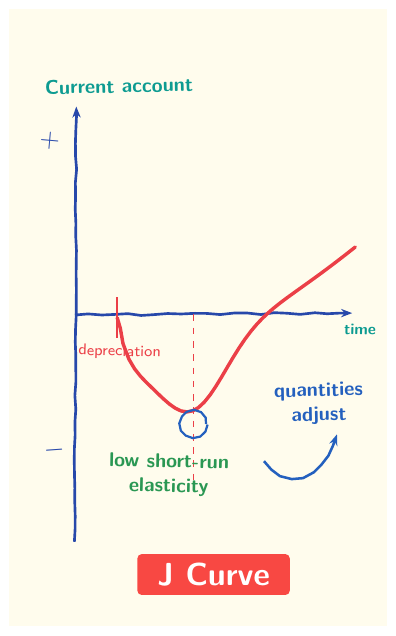
\includegraphics[height=0.70\textheight,keepaspectratio]{assets/j_curve_final.png}

  \vspace{0.2cm}
  \small
  GIF preview: \href{run:assets/j_curve_animation.gif}{open local animation preview}
\end{frame}

\begin{frame}{Reusable Pattern Added}
  \begin{itemize}[<+->]
    \item Generalized from one trade example into \textbf{delayed adjustment paths}.
    \item Works for macro response lags, exchange-rate J-curves, marketing wear-in, adoption, process learning, and recovery curves.
    \item Required structure: time axis, intervention marker, baseline, short-run friction, eventual catch-up or new steady state.
  \end{itemize}
\end{frame}

\section{Research Figures}

\begin{frame}{Belief Corridor / Survival Region}
  \centering
  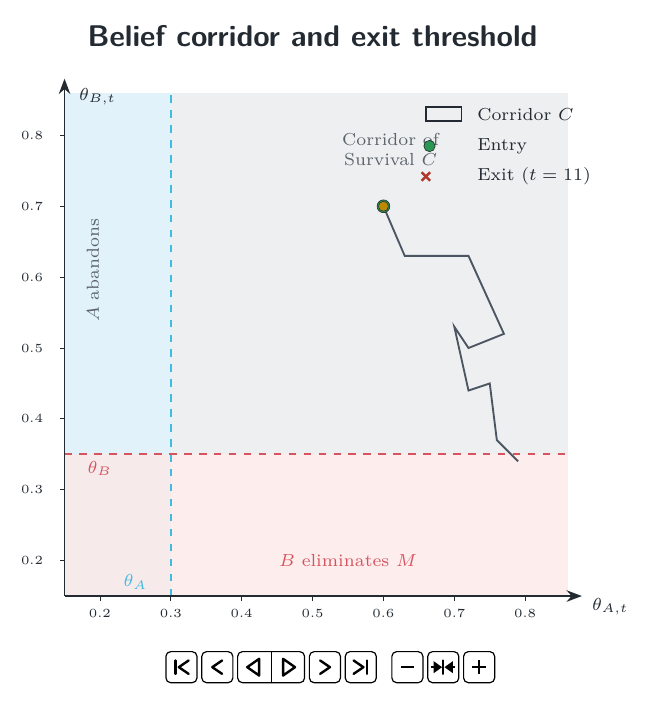
\includegraphics[width=\linewidth,height=0.72\textheight,keepaspectratio]{assets/belief_corridor_final.png}

  \vspace{0.2cm}
  \small
  GIF preview: \href{run:assets/belief_corridor_animation.gif}{open local animation preview}
\end{frame}

\begin{frame}{NBER Figure Adaptation}
  \begin{columns}[T,totalwidth=\textwidth]
    \begin{column}{0.46\textwidth}
      \textbf{Input figure screenshot}

      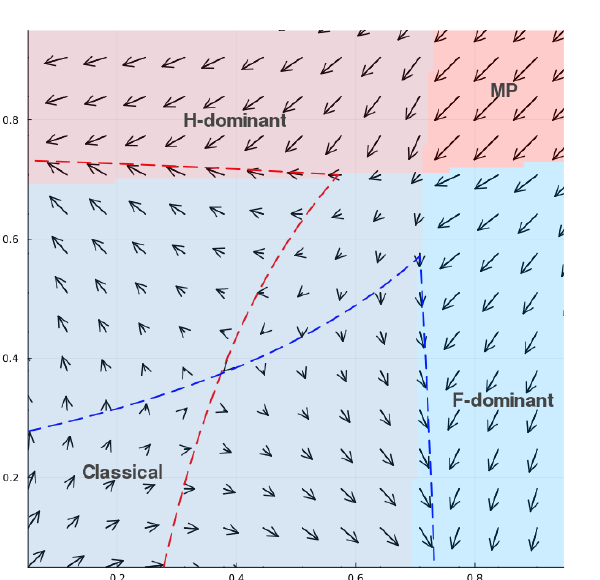
\includegraphics[width=\linewidth,height=0.58\textheight,keepaspectratio]{assets/nber_input.png}
    \end{column}
    \begin{column}{0.50\textwidth}
      \textbf{Animated schematic adaptation}

      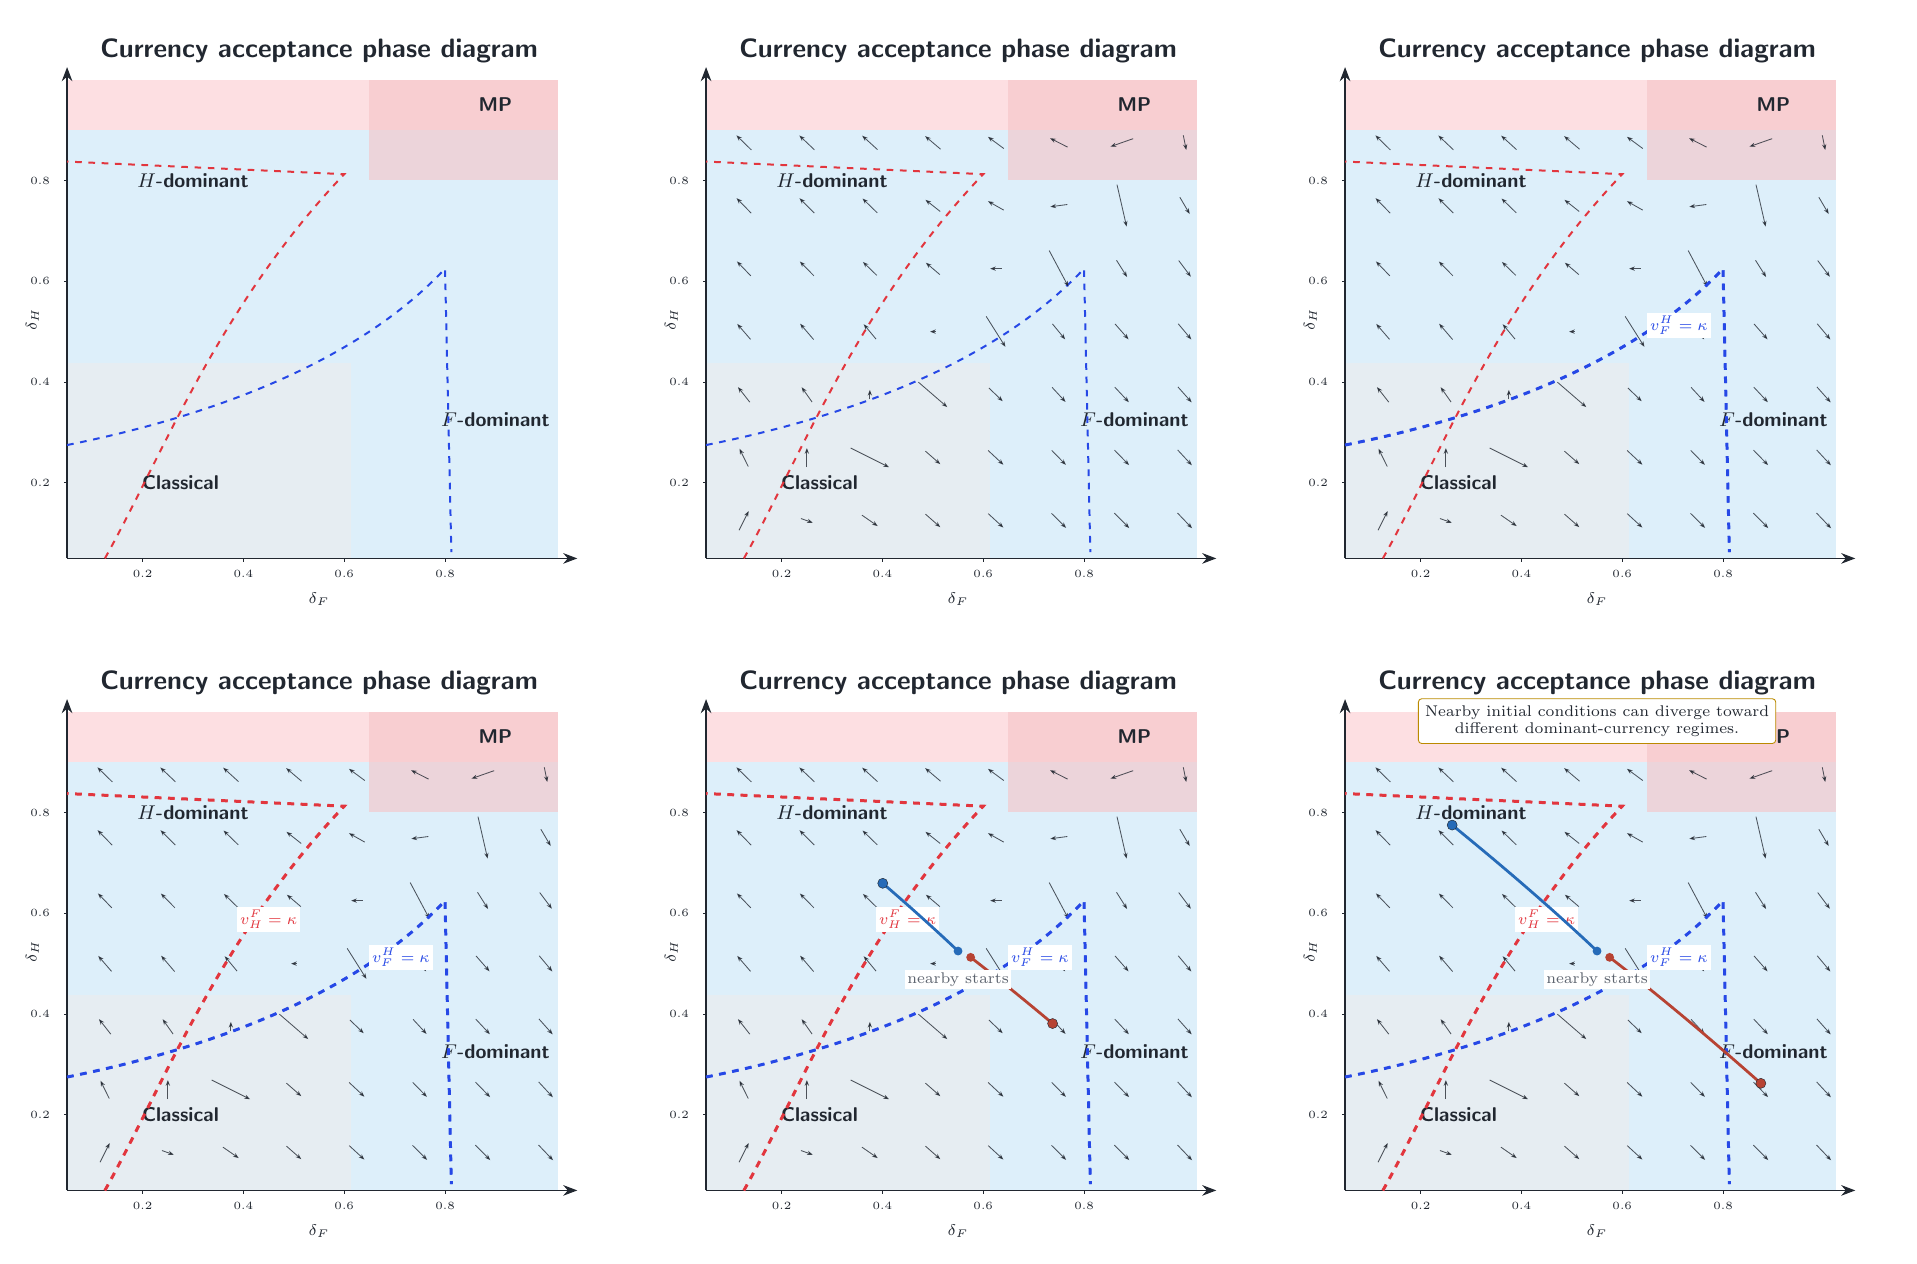
\includegraphics[width=\linewidth,height=0.58\textheight,keepaspectratio]{assets/nber_animation_contact.png}
    \end{column}
  \end{columns}
\end{frame}

\begin{frame}{Research-Figure Lessons}
  \begin{itemize}[<+->]
    \item Be explicit when a figure is a schematic adaptation rather than numerical reproduction.
    \item Animate nullclines, vector fields, and trajectories only when the motion explains a mechanism.
    \item If a smooth/vector-field version hits TeX memory limits, reduce redundant density or stitch segments.
  \end{itemize}
\end{frame}

\section{Animation QA}

\begin{frame}{Game Tree: Pacing Gate}
  \centering
  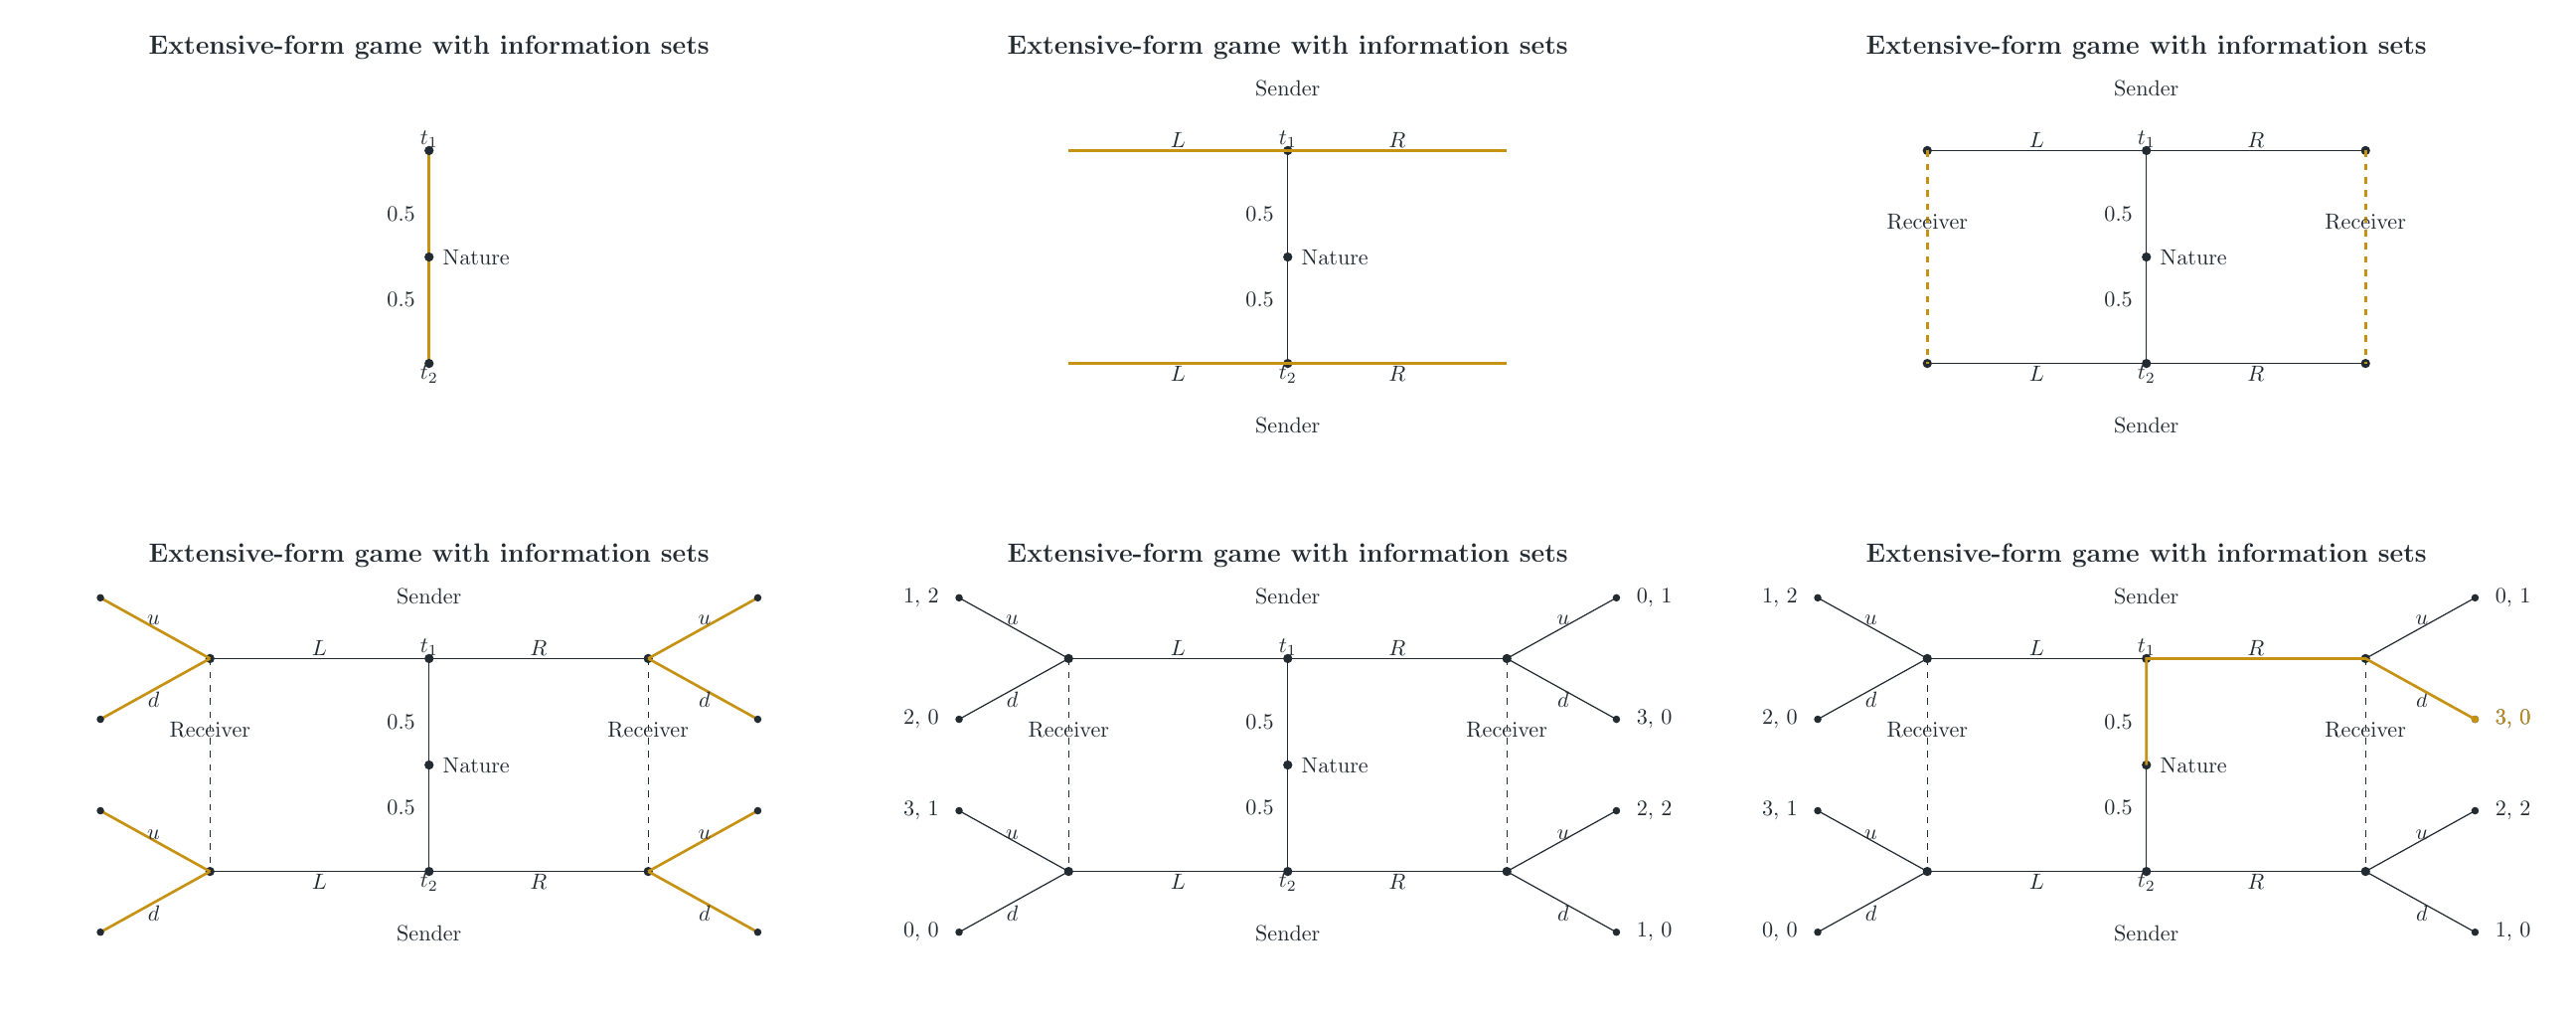
\includegraphics[width=\linewidth,height=0.74\textheight,keepaspectratio]{assets/game_tree_contact.png}
\end{frame}

\begin{frame}{Macro Cycle: Smooth Fill}
  \centering
  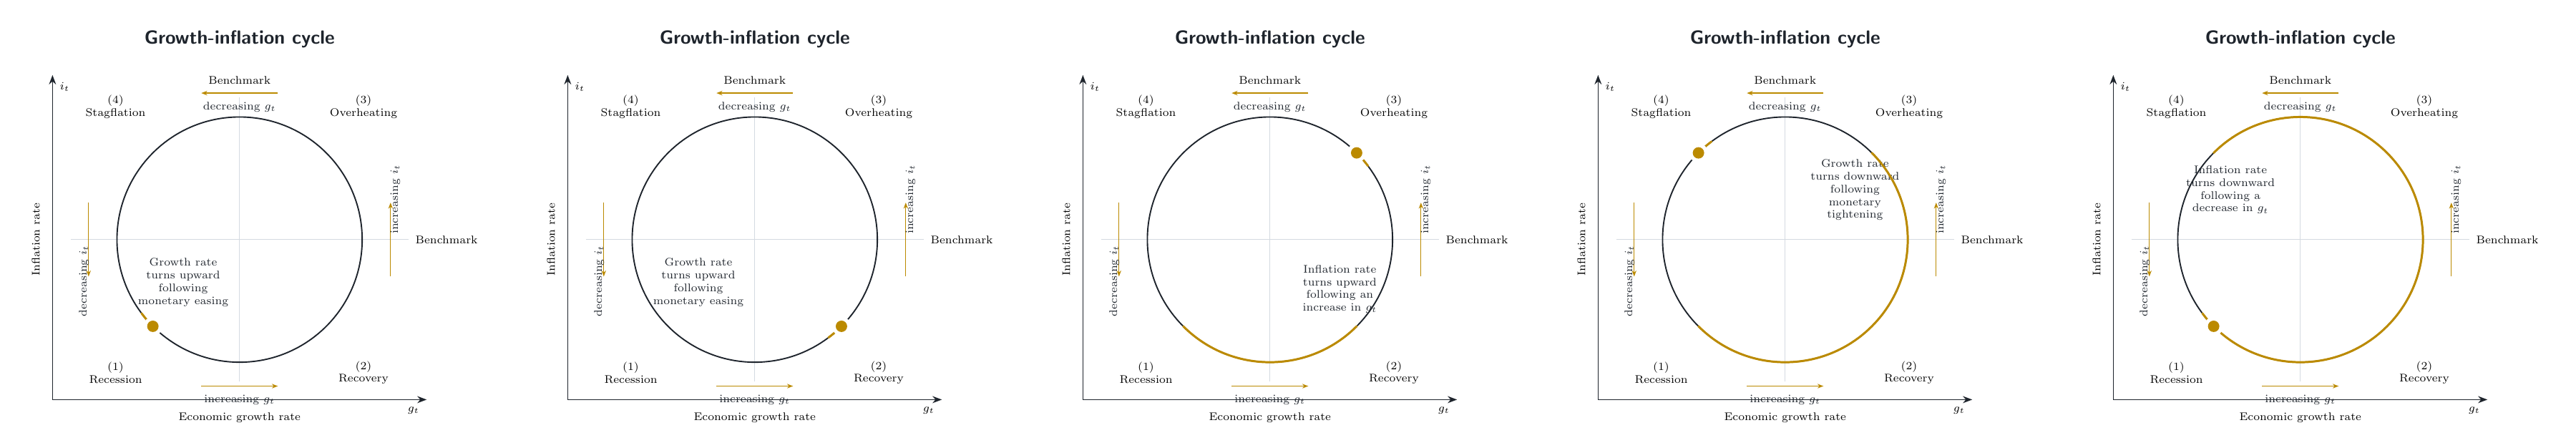
\includegraphics[width=\linewidth,height=0.74\textheight,keepaspectratio]{assets/macro_cycle_contact.png}
\end{frame}

\begin{frame}{What Changed in the Skill}
  \begin{itemize}[<+->]
    \item Ask what changes over time before writing animation code.
    \item Use pacing holds for dense frames, threshold crossings, payoffs, legends, and final states.
    \item Ask before expensive smooth renders when a stepped preview would answer the question.
    \item Keep captions outside standalone images by default.
    \item Preserve versioned outputs during critique to avoid stale render confusion.
  \end{itemize}
\end{frame}

\section{Package}

\begin{frame}{Repository Package}
  \small
  \begin{itemize}[<+->]
    \item \texttt{skills/tikz-diagrams/SKILL.md}: canonical agent skill.
    \item \texttt{scripts/}: deterministic checks, renderers, contact sheets, and animation previews.
    \item \texttt{references/}: visual QA, patterns, animation workflow, critique, and clean-room tests.
    \item \texttt{AGENTS.md}, \texttt{CLAUDE.md}, \texttt{GEMINI.md}, Copilot instructions, and Cursor rules.
    \item \texttt{README.md}: human install and dependency notes.
  \end{itemize}
\end{frame}

\begin{frame}{Practical Safety Bar}
  \begin{itemize}[<+->]
    \item Agents should ask before installing missing dependencies.
    \item The public skill copy should not include local absolute paths or personal output folders.
    \item The local working copy can keep local quality baselines and regression fixtures.
    \item Rendered examples are demos; the source skill remains the reusable artifact.
  \end{itemize}
\end{frame}

\end{document}
